
\section{Cartpole}
Cartpole is a pre-built environment from the gym library, therefore, it just has to be imported using:
\begin{center}
    gym.make('CartPole-v1')
\end{center}

In this experiment the version 1 was prefered over version 0 as it provides more timesteps, setting the limit to 500 timesteps per episode.

There are three main parts in stage 1:
\begin{figure}[H]
    \centering
    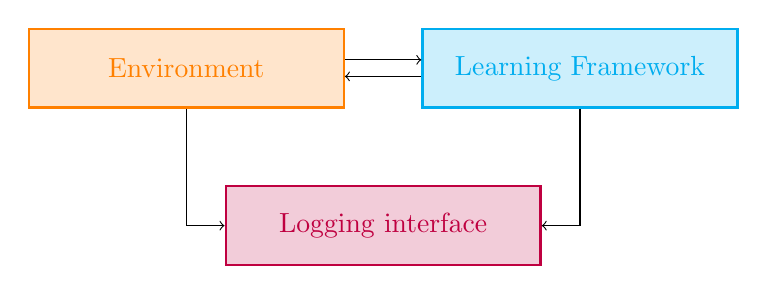
\begin{tikzpicture}
        \node[rectangle, 
        draw, 
        thick,
        minimum width = 4cm,
        minimum height = 1cm,
        color=orange,
        fill=orange!20,
        ] (A) at (0,0)  {Environment};
        \node[rectangle, 
        draw, 
        thick,
        minimum width = 4cm,
        minimum height = 1cm,
        color=cyan,
        fill=cyan!20,
        ] (B) at (5,0)  {Learning Framework};
        \node[rectangle, 
        draw, 
        thick,
        minimum width = 4cm,
        minimum height = 1cm,
        color=purple,
        fill=purple!20,
        ] (C) at (2.5,-2)  {Logging interface};

        \draw[->] ([yshift=3]A.east) -- ([yshift=3]B.west);
        \draw[<-] ([yshift=-3]A.east) -- ([yshift=-3]B.west);
        \draw[->] (B.south) |- (C.east);
        \draw[->] (A.south) |- (C.west);

        
    \end{tikzpicture}
\end{figure}

Each of this should interact for a successfull implementation of the first stage.
After the environment is imported, the learning framework is imported, this is a framework that is used to train the agent.
In this stage, two main implementations were explred, Keras-rl and a manual implementation of the keras API.

    \subsection*{Keras-rl}
    To implement keras-rl\cite{kerasrl2} in the specific hardware used in this project, it was required to be installed from source inside a miniforge environment.
    To be able to setup the model used by keras-rl tensorflow was required, once again, the hardware required a custom installation, the instructions can be found on the manufactures website \cite{apple-tf}.

    As the requirements were met, the next step is to setup a model, this was setup using keras, imported from tensorflow.
    \pagebreak
    \lstset{language=Python}
    \lstset{frame=lines}
    \lstset{caption={Setting up the model in the cartpole environment}}
    \lstset{label={lst:code_direct}}
    \lstset{basicstyle=\footnotesize}
    \begin{lstlisting}
        from tensorflow.keras.models import Sequential
        from tensorflow.keras.layers import Dense, Flatten, Input
        from tensorflow.keras.optimizers import Adam

        states = env.observation_space.shape
        actions = env.action_space.n

        def build_model(states, actions):
            model = Sequential() 
            model.add(Input(states))
            model.add(Flatten())
            model.add(Dense(12, activation='relu', input_shape=(1,4)))
            model.add(Dense(12, activation='relu'))
            model.add(Dense(actions, activation='linear'))
            return model

        model = build_model(states, actions)
        model.build(states)
    \end{lstlisting}

    The code displayed above is used to import the required packages for the model, proceeded by a function where the model is defined, here, we can see that the model receives the inputs, flattens this followed by a fully connected layer with 12 neurons and relu activation function,
    this layer is followed by another fully connected layer with 12 neurons and relu activation function.



\section{2D Walker}
The 2d environment uses as a physics engine Pymunk \cite{pymunk}, a python implementation of Chipmunk\cite{chipmunk} 
in conjunction with pygame \cite{pygame} to render the simulation. 
%extend the decision of pygame and pymunk in this paragraph ^

\section{3D Walker}

